\documentclass[12pt]{article}

% Настройка русского языка и шрифтов
\usepackage[utf8]{inputenc}
\usepackage[russian]{babel}
\usepackage[T2A]{fontenc}

% Математические пакеты
\usepackage{amsmath, amssymb, amsfonts}

% Настройка страницы
\usepackage{geometry}
\geometry{a4paper, margin=0.8in}

% Другие полезные пакеты
\usepackage{hyperref}
\usepackage{booktabs}
\usepackage{enumitem}
\usepackage{longtable}
\usepackage{graphicx}
\usepackage{xcolor}

% Определение стилей для комментариев
\definecolor{commentgray}{rgb}{0.4,0.4,0.4}
\definecolor{antigravityblue}{rgb}{0.0, 0.45, 0.74}

\newcommand{\commentary}[1]{{\small\itshape\color{commentgray} #1}}
\newcommand{\antigravity}[1]{{\small\color{antigravityblue}\textbf{Antigravity:} #1}}

% Настройка ссылок
\hypersetup{
    colorlinks=true,
    linkcolor=blue,
    filecolor=magenta,      
    urlcolor=cyan,
    pdftitle={Глубокий разбор: Подбор гиперпараметров},
}


\begin{document}

\subsection{Подбор гиперпараметров: определение}
В машинном обучении различают два типа переменных:
\begin{itemize}
    \item \textbf{Параметры модели:} это веса, которые алгоритм находит самостоятельно в процессе обучения на данных (например, коэффициенты $w$ в линейной регрессии).
    \item \textbf{Гиперпараметры:} это внешние настройки алгоритма, которые задаются исследователем \textbf{до} начала обучения. Они определяют саму структуру модели и способ её обучения (например, глубина дерева, количество соседей в KNN, сила регуляризации).
\end{itemize}


\commentary{Подбор гиперпараметров — это процесс поиска таких значений, при которых модель показывает наилучшее качество на новых данных.}

\subsection{Ключевые гиперпараметры для популярных алгоритмов}

Ниже приведен перечень основных гиперпараметров, которые чаще всего настраиваются для достижения лучшего качества моделей.

\begin{description}
    \item[Линейные модели (Linear/Logistic Regression):]
    \begin{itemize}
        \item \texttt{C} или \texttt{alpha}: Коэффициент регуляризации. Чем меньше значение (для C), тем сильнее регуляризация.
        \item \texttt{penalty}: Тип штрафа (\texttt{l1}, \texttt{l2}, \texttt{elasticnet}).
        \item \texttt{solver}: Алгоритм оптимизации (\texttt{liblinear}, \texttt{saga}, \texttt{lbfgs}).
    \end{itemize}

    \item[Метод k-ближайших соседей (k-NN):]
    \begin{itemize}
        \item \texttt{n\_neighbors}: Число соседей $k$.
        \item \texttt{weights}: Весовая функция (\texttt{uniform} или \texttt{distance}).
        \item \texttt{p}: Параметр метрики Минковского (1 — Манхэттен, 2 — Евклид).
    \end{itemize}

    \item[Деревья решений (Decision Trees):]
    \begin{itemize}
        \item \texttt{max\_depth}: Максимальная глубина дерева (контроль переобучения).
        \item \texttt{min\_samples\_split}: Минимум объектов, необходимых для разделения узла.
        \item \texttt{min\_samples\_leaf}: Минимум объектов в листе.
        \item \texttt{criterion}: Критерий ветвления (\texttt{gini}, \texttt{entropy}).
    \end{itemize}

    \item[Случайный лес (Random Forest):]
    \begin{itemize}
        \item \texttt{n\_estimators}: Количество деревьев в лесу.
        \item \texttt{max\_features}: Число признаков для поиска лучшего разбиения.
        \item *Плюс все параметры одиночного дерева.*
    \end{itemize}

    \item[Градиентный бустинг (XGBoost, LightGBM, CatBoost):]
    \begin{itemize}
        \item \texttt{learning\_rate}: Скорость обучения (шаг градиентного спуска).
        \item \texttt{n\_estimators}: Количество итераций (деревьев).
        \item \texttt{max\_depth}: Глубина деревьев.
        \item \texttt{subsample}: Доля выборки для обучения одного дерева.
        \item \texttt{reg\_alpha} / \texttt{reg\_lambda}: L1 и L2 регуляризация.
    \end{itemize}

    \item[Метод опорных векторов (SVM):]
    \begin{itemize}
        \item \texttt{C}: Параметр штрафа за ошибки (баланс между отступом и точностью).
        \item \texttt{kernel}: Тип ядра (\texttt{linear}, \texttt{rbf}, \texttt{poly}).
        \item \texttt{gamma}: Коэффициент для нелинейных ядер.
    \end{itemize}

    \item[Нейронные сети:]
    \begin{itemize}
        \item \texttt{learning\_rate}: Скорость обучения.
        \item \texttt{batch\_size}: Размер пакета данных.
        \item \texttt{optimizer}: Алгоритм оптимизации (\texttt{Adam}, \texttt{SGD}, \texttt{RMSprop}).
        \item \texttt{dropout\_rate}: Коэффициент исключения нейронов (регуляризация).
    \end{itemize}
\end{description}


\subsection{Методология подбора}
Чтобы оценка качества была честной, нельзя подбирать гиперпараметры на тех же данных, на которых модель обучается или на которых она окончательно тестируется.

\subsubsection{Схема Train-Validation-Test}
Классический подход подразумевает разделение всего датасета на три независимые части. Это необходимо, чтобы избежать «переобучения под тест»: если мы будем подбирать параметры, ориентируясь на тестовую выборку, мы получим слишком оптимистичную оценку, которая не подтвердится на реальных данных (эффект "подгонки" под тест).

\begin{itemize}
    \item \textbf{Train (Обучающая):} ~60--80\% данных. Используется исключительно для настройки внутренних весов модели (параметров).
    \item \textbf{Validation (Валидационная):} ~10--20\% данных. Служит для оценки качества при разных гиперпараметрах. Именно по результатам на этой части мы выбираем лучший набор настроек.
    \item \textbf{Test (Тестовая):} ~10--20\% данных. «Золотой стандарт» оценки. К этой части обращаются ровно один раз в самом конце. 
\end{itemize}

\commentary{Важное правило: если после оценки на Test вы решили «еще немного подкрутить» параметры, Test автоматически становится частью Validation, и вам нужны новые данные для честного финального теста.}

\textbf{Типичный процесс подбора:}
\begin{enumerate}
    \item Фиксируем конкретный набор гиперпараметров.
    \item Обучаем модель на \textbf{Train}.
    \item Замеряем метрику качества на \textbf{Validation}.
    \item Повторяем шаги 1--3 для всех интересующих комбинаций.
    \item Выбираем комбинацию с лучшим результатом на валидации.
    \item (Опционально) Переобучаем финальную модель на объединенной выборке \textbf{Train + Validation}.
    \item Делаем итоговый замер качества на \textbf{Test}.
\end{enumerate}

\begin{figure}[h]
	\centering
	\begin{minipage}{0.48\textwidth}
		\centering
		
\includegraphics[width=\textwidth]{train_val_test.png}
		\caption{Схема разделения данных для честной оценки.}
		\label{fig:split}
	\end{minipage}
	\hfill
	\begin{minipage}{0.48\textwidth}
		\centering
		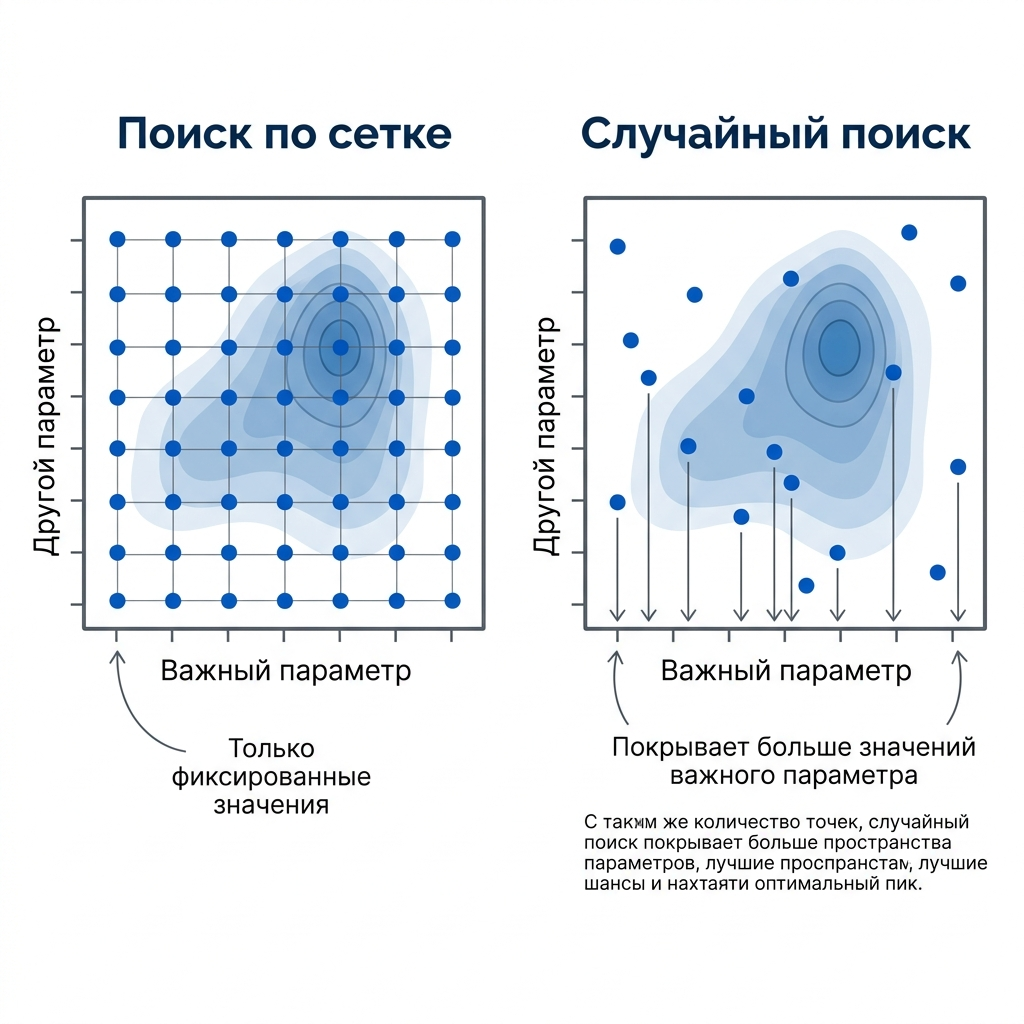
\includegraphics[width=\textwidth]{grid_vs_random.png}
		\caption{Сравнение Grid Search и Random Search.}
		\label{fig:search}
	\end{minipage}
\end{figure}

\subsection{Кросс-валидация (k-Fold)}
Если данных недостаточно для выделения отдельной валидационной выборки или мы хотим получить более устойчивую оценку качества, используется \textbf{k-Fold кросс-валидация}.

\textbf{Принцип работы:}
\begin{enumerate}
    \item Обучающая выборка делится на $k$ равных частей (фолдов).
    \item Модель обучается $k$ раз. В каждой итерации один фолд используется как валидационный, а остальные $k-1$ — как обучающие.
    \item Итоговая метрика — это среднее арифметическое результатов на всех $k$ валидационных фолдах.
\end{enumerate}

\begin{itemize}
    \item \textbf{Stratified k-Fold:} Вариант для классификации, где в каждом фолде сохраняется то же процентное соотношение классов, что и во всей выборке. Это критично при сильном дисбалансе классов.
    \item \textbf{Плюсы:} Более надежная оценка качества (низкая дисперсия метрики), использование всех данных и для обучения, и для валидации.
    \item \textbf{Минусы:} Вычислительная сложность (модель нужно обучить $k$ раз).
\end{itemize}

\subsection{Grid Search (Поиск по сетке)}
\textbf{Принцип:} Исследователь задает дискретный список значений для каждого гиперпараметра. Алгоритм строит декартово произведение этих списков и перебирает \textbf{абсолютно все возможные комбинации}.

\begin{itemize}
    \item \textbf{Плюсы:} 
    \begin{itemize}
        \item Исчерпывающий поиск в заданных границах.
        \item Простота интерпретации и воспроизводимость.
    \end{itemize}
    \item \textbf{Минусы:} 
    \begin{itemize}
        \item «Проклятие размерности»: количество комбинаций растет экспоненциально с добавлением новых параметров.
        \item Неэффективность: много времени тратится на перебор «неважных» параметров, которые слабо влияют на результат.
    \end{itemize}
\end{itemize}

\subsection{Random Search (Случайный поиск)}
\textbf{Принцип:} Вместо фиксации сетки мы задаем распределения (например, равномерное или логарифмическое) для параметров. Значения выбираются случайно.

\textbf{Почему это работает (согласно Bergstra \& Bengio):} В большинстве задач лишь небольшое количество гиперпараметров являются действительно важными. Grid Search тратит время на перебор неважных измерений. Random Search же исследует гораздо больше уникальных значений «важных» параметров за то же количество итераций.

\begin{itemize}
    \item \textbf{Плюсы:} 
    \begin{itemize}
        \item Значительно быстрее при большом количестве параметров.
        \item Не привязан к конкретному шагу сетки.
        \item Вероятностная гарантия: при $n=60$ итерациях мы с вероятностью 95\% найдем решение, входящее в топ-5\% лучших в пространстве поиска.
    \end{itemize}
    \item \textbf{Минусы:} 
    \begin{itemize}
        \item Не гарантирует нахождение глобального максимума (может «промахнуться» мимо узкого пика).
        \item Результат зависит от случайности (нужен фиксированный \texttt{random\_state}).
    \end{itemize}
\end{itemize}


\subsection{Продвинутые методы подбора}

Когда Grid и Random Search становятся слишком дорогими, на помощь приходят адаптивные методы, которые «учатся» на результатах предыдущих итераций.

\subsubsection{Байесовская оптимизация}
Основная идея — не искать вслепую, а построить вероятностную модель зависимости целевой метрики от гиперпараметров.

\begin{itemize}
    \item \textbf{Суррогатная модель (Surrogate Model):} Аппроксимирует реальную (дорогую) целевую функцию. Чаще всего используются \textit{Гауссовские процессы} или \textit{Random Forest}. Модель предсказывает не только среднее значение метрики в точке $x$, но и дисперсию (неопределенность) $\sigma(x)$.
    \item \textbf{Функция полезности (Acquisition Function):} Решает, какую точку исследовать следующей. Она балансирует между:
    \begin{itemize}
        \item \textit{Exploitation} (Эксплуатация): Проверка областей, где модель предсказывает высокий результат.
        \item \textit{Exploration} (Исследование): Проверка областей с высокой неопределенностью (где мы еще не были).
    \end{itemize}
    \item \textbf{Популярные функции:} \textbf{EI} (Expected Improvement) — математическое ожидание улучшения, \textbf{UCB} (Upper Confidence Bound) — верхняя граница доверительного интервала.
\end{itemize}

\subsubsection{Алгоритм TPE (Tree-structured Parzen Estimator)}
Это «облегченный» и эффективный вариант байесовской оптимизации, используемый в Optuna и Hyperopt. 

\textbf{Интуиция:} Вместо моделирования функции $P(y|x)$ (как в Гауссовских процессах), TPE моделирует плотность распределения параметров $P(x|y)$. 
\begin{enumerate}
    \item Все результаты делятся на две группы: «лучшие» (верхний квантиль) и «остальные».
    \item Строятся два распределения: $l(x)$ для лучших и $g(x)$ для остальных.
    \item Следующей выбирается точка, которая максимизирует отношение $l(x)/g(x)$ — то есть точка, которая с наибольшей вероятностью принадлежит к «хорошим» результатам и с наименьшей — к «плохим».
\end{enumerate}

\subsubsection{Population Based Training (PBT)}
Метод, вдохновленный эволюцией, идеально подходит для тяжелых нейросетей. В отличие от других методов, PBT подбирает параметры \textbf{прямо в процессе обучения}, а не запускает обучение заново.

\begin{itemize}
    \item \textbf{Exploit:} Слабые модели в популяции «умирают», копируя веса более успешных соседей.
    \item \textbf{Explore:} После копирования весов гиперпараметры модели-победителя слегка мутируют (добавляется шум), чтобы найти еще более удачную комбинацию.
    \item \textbf{Результат:} Мы получаем и обученную модель, и оптимальное расписание (schedule) изменения параметров (например, learning rate) за один проход.
\end{itemize}

\subsubsection{Hyperband и Successive Halving}
Эти алгоритмы фокусируются на эффективном распределении ресурсов (времени, данных).
\begin{itemize}
    \item \textbf{Принцип:} Мы запускаем много конфигураций на очень малом количестве итераций.
    \item \textbf{Отсев:} После каждой стадии выживает только топ-$1/n$ лучших конфигураций, которым выделяется в $n$ раз больше ресурсов.
    \item Это позволяет быстро отбросить явно плохие архитектуры и сосредоточиться на перспективных.
\end{itemize}

\begin{figure}[h]
    \centering
    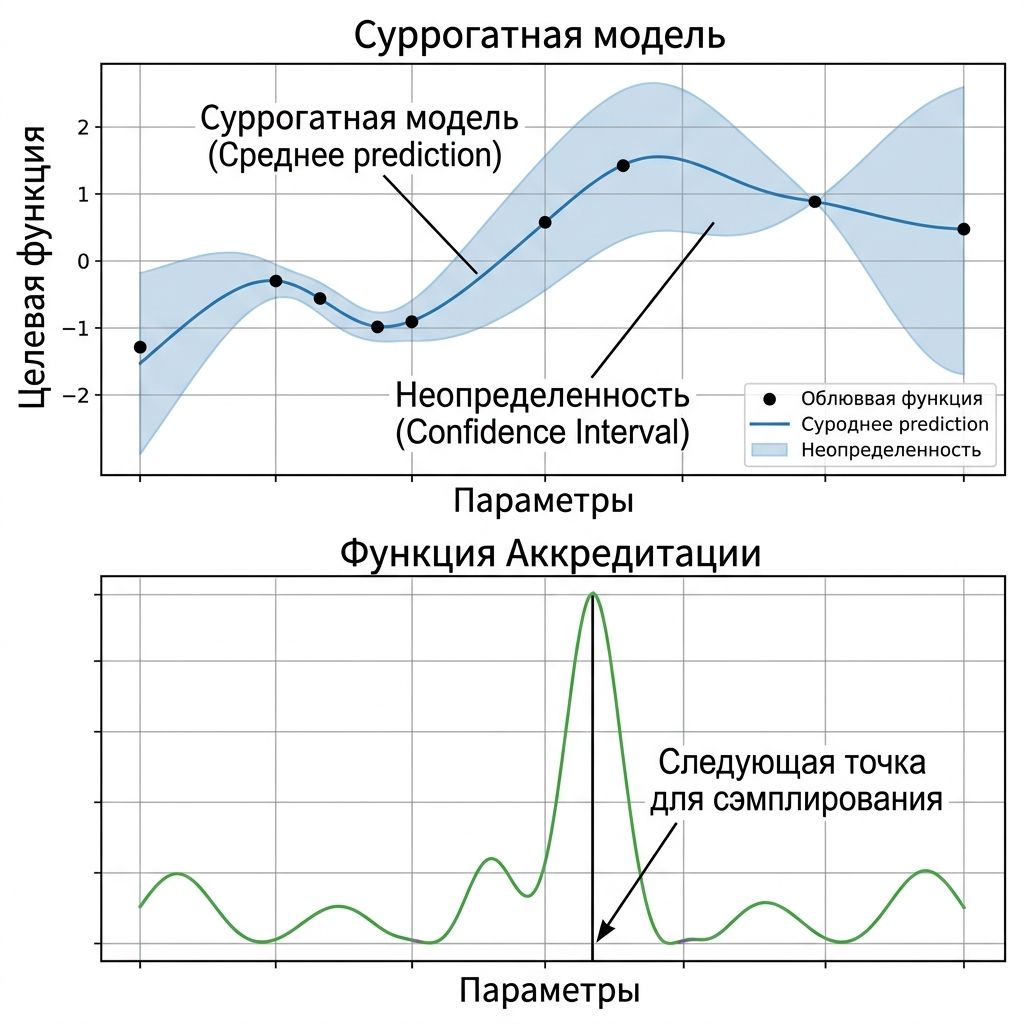
\includegraphics[width=0.7\textwidth]{bayesian_opt.png}
    \caption{Интуиция байесовской оптимизации.}
\end{figure}

\subsection{Опенсорс-библиотеки и инструменты}

Выбор инструмента зависит от сложности модели и имеющихся вычислительных ресурсов.

\begin{longtable}{lp{0.65\textwidth}}
\toprule
\textbf{Библиотека} & \textbf{Ключевые особенности и алгоритмы} \\
\midrule
\textbf{Scikit-learn} & \textbf{Базовый стандарт.} Предлагает \texttt{GridSearchCV} и \texttt{RandomizedSearchCV}. В новых версиях появился \texttt{HalvingGridSearchCV}, который использует метод последовательных сокращений (Successive Halving) для быстрой отбраковки плохих комбинаций. \\
\midrule
\textbf{Optuna} & \textbf{Лидер индустрии.} Использует подход \textit{Define-by-run} (пространство поиска описывается прямо внутри функции). \\
& \textbullet{} \textbf{Pruning:} Автоматически останавливает «безнадежные» итерации (trial), не дожидаясь конца обучения. \\
& \textbullet{} \textbf{Алгоритмы:} TPE, CMA-ES, Random Search. Отличная визуализация важности параметров. \\
\midrule
\textbf{Hyperopt} & Классическая библиотека, популяризировавшая алгоритм \textbf{TPE} (Tree-structured Parzen Estimator). Имеет чуть более сложный синтаксис по сравнению с Optuna, но всё еще широко используется. \\
\midrule
\textbf{Scikit-Optimize} & Специализируется на \textbf{байесовской оптимизации}. Главный плюс — наличие \texttt{BayesSearchCV}, который можно использовать как прямую замену стандартным методам из sklearn. \\
\midrule
\textbf{Ray Tune} & Инструмент для \textbf{масштабируемого} подбора. Идеален для распределенных систем и тяжелых нейросетей. Поддерживает продвинутые стратегии, такие как \textbf{PBT} (Population Based Training) и Hyperband. \\
\midrule
\textbf{Keras Tuner} & Специализированное решение для экосистемы TensorFlow/Keras. Позволяет подбирать не только параметры, но и саму архитектуру нейросети (количество слоев, фильтров и т.д.). \\
\bottomrule
\end{longtable}

\antigravity{Начинай всегда с Random Search, чтобы быстро прощупать почву. Если задача критически важна — переходи на Optuna.}

\end{document}
